\chapter{Convertidores de Aproximaciones Sucesivas}

El algoritmo de aproximaciones sucesivas ofrece un buen compromiso entre velocidad y complejidad, y es el más frecuente cuando no se trata de obtener una exactitud muy elevada. Hay muchos modelos de 8, 10, 12, 14 y 16 bits, con tiempos de conversión entre 1 y 100$\mu$s. Se puede montar con componentes discretos, pero su coste supera el de muchos de los CI disponibles.

El método consiste en ir comparando la tensión de entrada con una tensión analógica generada internamente con un CDA, cuya entrada digital incrementa o decrementa según que el resultado de la comparación indique, respectivamente, que la tensión de entrada es inferior o superior a la tensión generada internamente. Los errores del CDA pueden llevar a no linealidades.

El tiempo de conversión aumenta al hacerlo la resolución deseada, pero es independiente de la amplitud de la entrada. El límite actual es de unas $10^6$ conversiones para 12 bits. Dado que el resultado de una comparación no se fija en el registro de salida hasta que llega el ciclo del reloj siguiente a aquel en el que se ha efectuado la comparación, si la frecuencia de reloj es $f_r$ el tiempo de conversión para $n$ bits es:

\begin{equation}
    t_c = \frac{n + 1}{f_r}
\end{equation}

Un inconveniente de este método es su no linealidad si la entrada varía durante el tiempo de conversión. Para evitar que la entrada cambie durante la conversión, se precede al CAD con un amplificador S\&H; esto no evita, sin embargo, que la muestra tomada pueda venir influida por el posible ruido en la entrada. En cualquier caso son, pues, convertidores muy susceptibles al ruido.

\begin{figure}[H]
     \centering
     \begin{subfigure}[b]{0.45\textwidth}
         \centering
         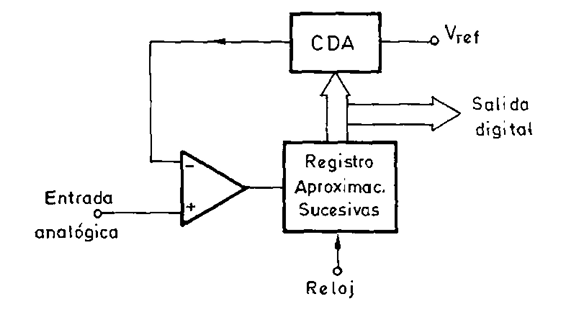
\includegraphics[width=\textwidth]{Imagenes/Convertidor de aproximaciones sucesivas.png}
         \caption{Esquema simplificado de un CAD basado en el algoritmo de aproximaciones sucesivas.}
     \end{subfigure}
     \hfill
     \begin{subfigure}[b]{0.45\textwidth}
         \centering
         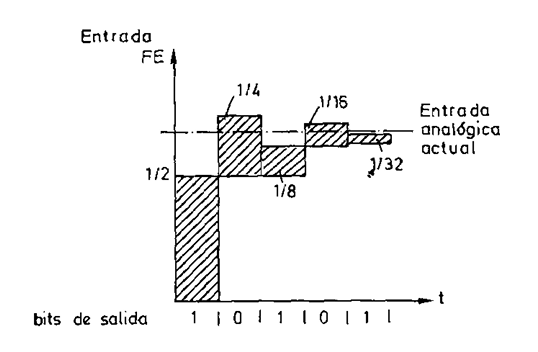
\includegraphics[width=\textwidth]{Imagenes/Convertidor Aproximaciones Sucesivas Bits.png}
         \caption{Asignación de valor a los bits de salida en comparaciones sucesivas.}
     \end{subfigure}
    \caption{}
\end{figure}